\documentclass[twocolumn]{article}

\usepackage[utf8]{inputenc}
\usepackage[spanish]{babel}
\usepackage{graphicx}
\usepackage{booktabs}
\usepackage{amsmath}
\usepackage{hyperref}
\usepackage{listings}
\usepackage[margin=2cm]{geometry}

\lstset{basicstyle=\ttfamily\footnotesize, breaklines=true, frame=single}

\title{Generacion de musica en ABC notation con un mini-GPT:\\ un estudio comparativo frente a un GRU}
\author{Ricardo Chaves \\ Deep Learning --- USFQ}
\date{}

\begin{document}
\maketitle

\begin{abstract}
Entrenamos un Transformer decoder pequeno (mini-GPT) a nivel de caracter para
generar melodias folk en ABC notation con acompanamiento de acordes, usando el
Nottingham Music Database. Comparamos el modelo contra una red recurrente
GRU como baseline en terminos de perplexity y de porcentaje de tunes
musicalmente validos (parseables con music21). A diferencia de un corpus de
melodias monofonicas, los tunes de Nottingham incluyen simbolos de acorde
(\texttt{"G"}, \texttt{"D7"}) y ritmos mas variados, por lo que el modelo aprende
a generar melodia y acordes de forma conjunta.
\end{abstract}

\section{Introduccion}
La generacion simbolica de musica puede plantearse como un problema de modelado
de lenguaje: la ABC notation representa una melodia como texto, por lo que
generar musica equivale a predecir el siguiente caracter dada la secuencia
previa. En este trabajo abordamos esa tarea y comparamos dos familias de modelos
vistas en el curso: redes recurrentes (GRU) y Transformers (GPT). El objetivo es
evaluar si la atencion captura mejor la estructura de largo alcance de un tune
(tonalidad, compas y forma AABB) que una RNN. El codigo y los modelos estan
disponibles en \url{https://github.com/ricardoch2296/deep_learning}.

\section{Trabajos relacionados}
El modelado de texto a nivel de caracter con RNN fue popularizado por
Karpathy~\cite{karpathy2015rnn}, quien mostro que un LSTM/GRU puede aprender
estructura de secuencias discretas. La GRU~\cite{cho2014gru} simplifica al LSTM
manteniendo buena memoria de largo plazo. El Transformer~\cite{vaswani2017attention}
reemplaza la recurrencia por auto-atencion, y GPT~\cite{radford2019language} lo
aplica al modelado causal de lenguaje. En musica, Sturm et
al.~\cite{sturm2016music} usaron RNN sobre ABC notation para componer melodias
folk, trabajo directamente relacionado con el nuestro.

\section{Metodologia}

\subsection{Datos}
Usamos el Nottingham Music Database~\cite{nottingham} en su version limpia de
jukedeck, una coleccion de melodias folk britanicas y americanas (jigs, reels,
valses, canciones) en ABC notation. A diferencia de un corpus monofonico, cada
tune trae \textbf{simbolos de acorde} entre comillas (p.ej. \texttt{"G"},
\texttt{"D7"}) sobre la melodia, ademas de silencios y compases variados. Cada
tune ya es un bloque ABC completo (cabecera + cuerpo); nos quedamos solo con los
que contienen acordes y filtramos por longitud (60--700 caracteres). El corpus
final tiene \texttt{992} tunes y \texttt{362K} caracteres, con un vocabulario de
\texttt{86} caracteres. Separamos 80/10/10 en train/val/test.

\subsection{Tokenizacion}
Tokenizamos a nivel de caracter (un entero por caracter unico). Es la
representacion mas simple y evita un vocabulario de sub-palabras, adecuado para
el conjunto reducido de simbolos de ABC.

\subsection{Modelos}
El \textbf{mini-GPT} es un \texttt{GPT2LMHeadModel} de HuggingFace con
$n_{layer}=6$, $n_{embd}=256$, $n_{head}=8$, contexto de 384 caracteres y
dropout 0.1, con \texttt{4.86M} parametros. El \textbf{baseline GRU} es un
\texttt{nn.Embedding} (128) seguido de una GRU de 2 capas (hidden 256) y una capa
lineal a vocabulario, con \texttt{0.72M} parametros. Ambos optimizan la misma
perdida de entropia cruzada sobre el siguiente caracter, para que la comparacion
sea justa.

\subsection{Entrenamiento}
Entrenamos por pasos (no epochs) dado el gran numero de ventanas. El GPT usa
AdamW ($lr=3\times10^{-4}$) con warmup y decaimiento coseno; el GRU usa Adam
($lr=2\times10^{-3}$). Guardamos el mejor checkpoint segun \texttt{val\_loss}.
El entrenamiento se realizo en una GPU NVIDIA H200.

\subsection{Evaluacion}
Reportamos \texttt{test\_loss} y perplexity ($\exp(\text{loss})$). Ademas, medimos
la \emph{validez musical}: generamos 100 tunes por modelo y contamos que fraccion
puede parsearse con music21~\cite{cuthbert2010music21} como una pieza con al menos
una nota.

\section{Resultados y discusion}

\begin{table}[t]
\centering
\begin{tabular}{lcccc}
\toprule
Modelo & params & test loss & perplexity & \% validos \\
\midrule
GPT & 4.86M & 1.093 & \textbf{2.98} & 99 \\
GRU & 0.72M & 1.165 & 3.21 & 100 \\
\bottomrule
\end{tabular}
\caption{Comparacion GPT vs GRU (test, temperatura 0.6).}
\label{tab:res}
\end{table}

\IfFileExists{figs/loss.png}{
\begin{figure}[t]
\centering
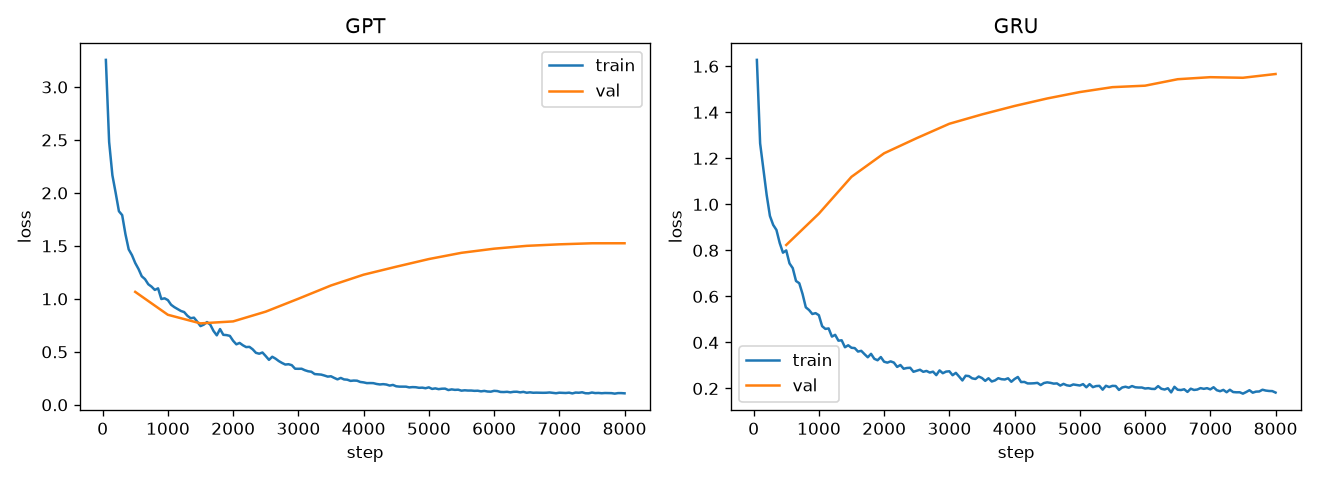
\includegraphics[width=\linewidth]{figs/loss.png}
\caption{Curvas de perdida (train/val) del GPT y el GRU.}
\label{fig:loss}
\end{figure}}{}

La Tabla~\ref{tab:res} resume los resultados. El mini-GPT obtiene una perplexity
menor (2.98 vs 3.21), lo que confirma que la auto-atencion modela mejor la
secuencia que la recurrencia del GRU, pese a que el GPT tiene mas parametros. La
Figura~\ref{fig:loss} muestra que ambos modelos convergen sin sobreajuste
marcado (train y val se mantienen juntas). En cambio, la metrica de validez
sintactica casi se satura: ambos modelos superan el 99\% de tunes parseables por
music21 a temperatura 0.6. Esto indica que aprender la \emph{sintaxis} de ABC
(incluyendo los acordes) es relativamente facil para las dos arquitecturas, y que
la validez sintactica no distingue calidad musical; la ventaja del GPT se ve en la
perplexity, no en la validez. Frente a un corpus monofonico, la perplexity aqui es
algo mayor porque el modelo tambien debe predecir los acordes, que anaden
incertidumbre.

\IfFileExists{figs/ablation_temp.png}{
\begin{figure}[t]
\centering
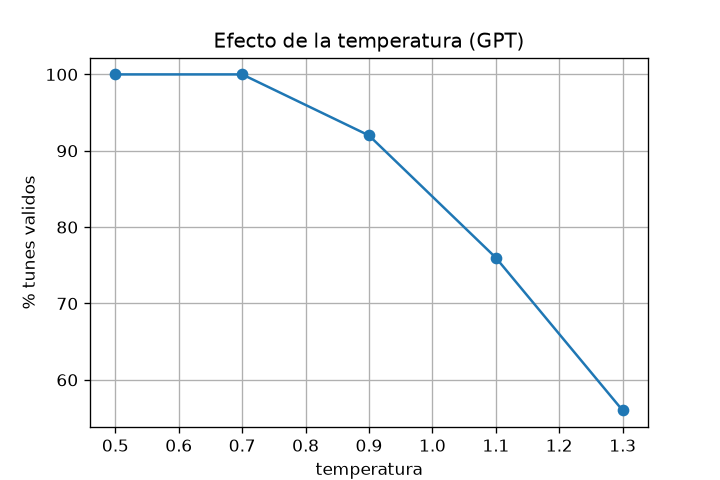
\includegraphics[width=\linewidth]{figs/ablation_temp.png}
\caption{Efecto de la temperatura de muestreo sobre el \% de tunes validos.}
\label{fig:temp}
\end{figure}}{}

La Figura~\ref{fig:temp} muestra el efecto de la temperatura: con valores bajos
(0.5--0.7) el GPT produce 100\% de tunes validos y mas conservadores, mientras que
al subir la temperatura (1.1--1.3) la validez cae (76\% y 56\%) porque aumenta la
diversidad a costa de producir texto mal formado. Por eso generamos con
temperatura 0.6.

El Listado~\ref{lst:tune} muestra un tune generado por el mini-GPT: respeta la
cabecera (compas y tonalidad), incluye \textbf{acordes} de acompanamiento
(\texttt{"D"}, \texttt{"G"}, \texttt{"A7"}) sobre la melodia y usa barras de
repeticion (\texttt{:| ::}), evidencia de que aprendio a generar melodia y armonia
de forma conjunta.

\begin{lstlisting}[caption={Tune generado por el mini-GPT (temperatura 0.6).},label=lst:tune]
X:1
T:The Brong The Gron
M:6/8
K:D
"D"d2A AFA|"D"d2d fga|"G"bag "A7"edc|"D"d3 d2::
A|"D"F2A AFA|"Bm"d2d "A"e2A|"Em"B2d "A7"efg|"D"fga "A7"bag|
"D"a2d AFA|"G"B2d "A7"efg|"D"aga "A7"gec|"D"d3 -d2:|
\end{lstlisting}

\section{Conclusiones}
Presentamos un generador de musica en ABC notation basado en un mini-GPT y lo
comparamos con un GRU. Usando el Nottingham Music Database, el modelo genera
melodias \textbf{con acordes de acompanamiento}, y el GPT logra menor perplexity
(2.98 vs 3.21), confirmando la ventaja de la atencion sobre la recurrencia para
modelar la estructura de un tune, mientras que ambos superan el 99\% de validez
sintactica. Entre las limitaciones estan el tamano reducido de los modelos y del
corpus, y que la validez sintactica no garantiza calidad musical (una mejor
evaluacion requeriria juicio humano o metricas musicales). Como mejoras futuras se
podrian usar tokenizacion por sub-unidades musicales, modelos mas grandes, o
condicionar la generacion por tipo de tune o tonalidad.

\bibliographystyle{plain}
\bibliography{refs}

\end{document}
